\documentclass[journal]{IEEEtran}

\usepackage[T1]{fontenc}
\usepackage[utf8]{inputenc}
\usepackage{amsmath,amssymb,amsfonts}
\usepackage{graphicx}
\usepackage{booktabs}
\usepackage{array}
\usepackage{url}
\usepackage{listings}
\usepackage{xcolor}
\usepackage[hidelinks]{hyperref}
\usepackage{orcidlink}
\usepackage{balance}

\graphicspath{{../figures/}}

\renewcommand{\topfraction}{0.92}
\renewcommand{\bottomfraction}{0.75}
\renewcommand{\textfraction}{0.08}
\renewcommand{\floatpagefraction}{0.80}

\lstset{
  basicstyle=\ttfamily\footnotesize, breaklines=true, columns=fullflexible,
  keepspaces=true, xleftmargin=1em, frame=single, framesep=4pt, rulecolor=\color{gray!50},
  backgroundcolor=\color{gray!6}, aboveskip=6pt, belowskip=4pt,
}

\begin{document}

\title{oreblocks: License-Free Synthetic Ore-Body\\ Block Models with a Stamped Exact\\ Ultimate-Pit Optimum}

\author{Felipe~Santiba\~nez-Leal~\orcidlink{0000-0002-0150-3246}%
\thanks{F. Santiba\~nez-Leal is with the CAOS open-research programme, Santiago, Chile
(e-mail: fsantibanez@gmail.com; ORCID 0000-0002-0150-3246).}%
\thanks{Software note, 2026. Package \texttt{oreblocks}; source (MIT) at
\url{https://github.com/fsantibanezleal/CAOS_OreBlocks}.}}

\markboth{Software Note, 2026}%
{Santiba\~nez-Leal: oreblocks, license-free synthetic ore-body block models with a stamped exact ultimate pit}

\maketitle

\begin{abstract}
Benchmarking an open-pit optimiser, a mine-dispatch simulator, or a teaching tool needs realistic ore-body block
models with a \emph{known} answer, but the standard public instances (the MineLib library) are granted for
academic download only and cannot be redistributed, and real mine models are proprietary. We present
\texttt{oreblocks}, a small pure-Python package that generates synthetic three-dimensional ore-body block models
of the \emph{same nature} as the public instances (seeded deposit archetypes with per-block grades, bench
structure, slope precedence and net-value economics) and stamps each one with its \emph{exact} ultimate-pit
optimum. The optimum is computed by the classical reduction of the ultimate-pit problem to a maximum closure and
thence to a minimum $s$--$t$ cut (Picard's theorem), solved by a Dinic max-flow with self-verifying closure and
value-identity checks, and every instance is emitted in exact MineLib \texttt{.blocks}/\texttt{.prec}/\texttt{.upit}
format with a sidecar carrying the stamped optimum, so any solver can be validated against a
known-by-construction answer without touching licensed data. We validate the solver \emph{independently} here:
on all four deposit archetypes its pit value agrees with a totally-unimodular linear program solved by a separate
method (SciPy HiGHS) to relative $10^{-15}$, i.e. to machine precision, and the exact solve runs in under a
second up to $32{,}000$ blocks. The package is deterministic, MIT-licensed, and consumed by downstream pit,
dispatch and haulage tools; every number and figure in this note regenerates from the committed artifacts.
\end{abstract}

\begin{IEEEkeywords}
Open-pit mining, ultimate pit limit, maximum closure, minimum cut, block model, MineLib, synthetic benchmark,
reproducible software, operations research.
\end{IEEEkeywords}

\section{Introduction}

\IEEEPARstart{T}{he} first question of open-pit mine planning is the \emph{ultimate pit}: given a
three-dimensional block model in which every block carries a net economic value (its recoverable metal minus the
cost to mine and process it) and a set of slope-precedence constraints (a block can be mined only after the
blocks above it in the pit wall), which set of blocks maximises total value while respecting the slopes? The
problem has a classical exact solution: Lerchs and Grossmann~\cite{lg} gave a graph algorithm in 1965, and
Picard~\cite{picard} showed that the ultimate pit is the maximum-value closure of the precedence graph, which is
the source side of a minimum $s$--$t$ cut and so is solvable exactly by any max-flow
algorithm~\cite{fordfulkerson,dinitz,hochbaumchen,hochbaum}. This is textbook operations
research~\cite{newman}, and any new pit optimiser, block-scheduling heuristic, or dispatch simulator wants to be
tested against it.

The obstacle is data. The community's shared benchmark, MineLib~\cite{minelib}, collects real and realistic
instances with published optima, but its instances are granted for academic download only and may not be
redistributed; real mine block models are proprietary. A developer who wants to ship a reproducible test suite, a
teaching notebook a student can run, or a continuous-integration job that certifies a solver against a known
answer, cannot bundle MineLib data and cannot use a real mine. What is missing is a way to \emph{generate}
instances of the same nature, with a known optimum, under a permissive license.

\texttt{oreblocks} fills that gap. It is a small pure-Python package that (i) generates seeded synthetic ore-body
block models from four geological archetypes, with per-block grades, bench structure, slope precedence and
net-value economics; (ii) solves each instance's ultimate pit \emph{exactly} by the maximum-closure/min-cut
reduction; and (iii) writes the instance in exact MineLib format with a sidecar carrying the stamped optimum, so
any downstream solver can be validated against a known-by-construction answer. Everything is deterministic given
a seed and every instance is clearly labelled synthetic. The one thing a synthetic benchmark must earn is trust
in its stamped answer, so we validate the solver \emph{independently} (Section~\ref{sec:validation}) against a
linear program solved by an entirely different method, finding agreement to machine precision.

\section{Statement of Need}\label{sec:need}

The users are developers and educators who need ore-body instances with ground truth and a license that permits
redistribution. A pit-optimisation library needs regression tests with known optima; a mine-dispatch or haulage
simulator (the downstream consumers of this package) needs geology-grounded scenarios rather than random
numbers; a course needs instances a student can generate and solve on a laptop. MineLib serves research but its
redistribution terms rule out all three, and real models are unavailable. \texttt{oreblocks} provides synthetic
instances of the same structure (three-dimensional benches, spatially-correlated grades, slope precedence, net
values) whose optimum is not looked up but \emph{computed exactly and stamped}, under the MIT license. The value
is a benchmark generator: not a single dataset but a seeded family, each member carrying its own certified
answer.

\section{Synthetic Ore Bodies}\label{sec:deposits}

An instance is a block grid (bench levels increasing upward, as in the published MineLib convention) carrying,
per block, a grade, a tonnage and a density. Grades come from a deterministic geological trend plus a
spatially-correlated (box-smoothed) random field, seeded so an instance is byte-identical given its
\texttt{(archetype, dims, seed)}. Four archetypes span the common deposit shapes: \texttt{porphyry} (a buried
ellipsoidal high-grade shell that yields broad bowl pits), \texttt{vein} (a dipping tabular zone giving narrow
steep pits), \texttt{layered} (horizontal stratabound bands), and \texttt{core\_halo} (a rich core inside a
low-grade halo). Each block's net value follows a standard mine-vs-process economics: revenue from recovered
metal at a price, less mining and processing costs, with the optimal destination (mill or waste) chosen per
block. Slope precedence is generated as a discrete cone (a block requires the pattern of blocks above it within a
slope angle), stored in the compressed-sparse-row layout MineLib's \texttt{.prec} format uses. The result is a
block model of the same nature as a real one, with the geology, the economics and the slope constraints that make
the ultimate-pit problem non-trivial.

\section{The Exact Ultimate-Pit Solver}\label{sec:solver}

\begin{figure*}[!t]
\centering
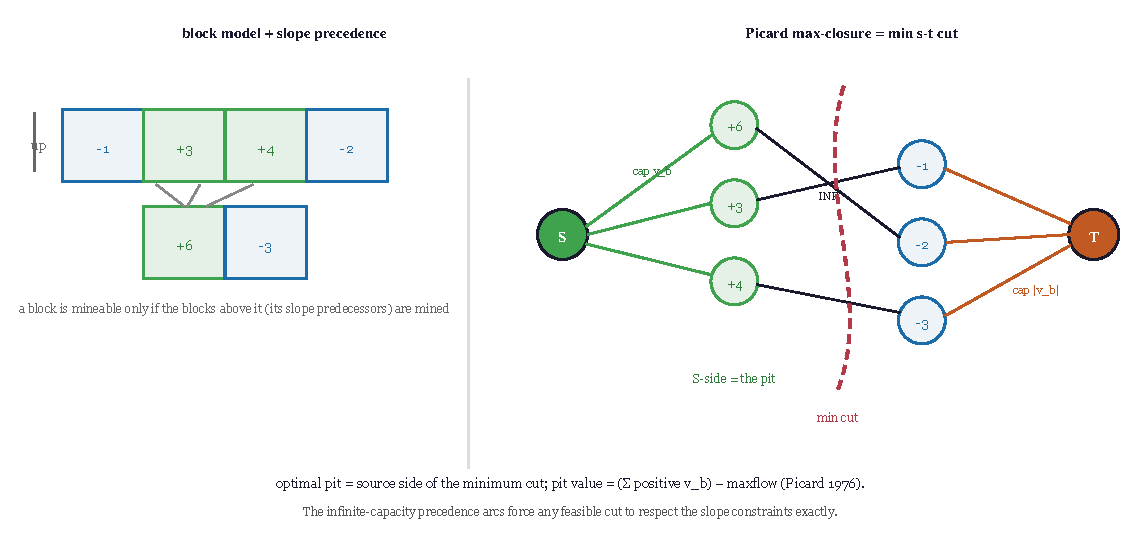
\includegraphics[width=0.99\textwidth]{fig-maxclosure.pdf}
\caption{The exact ultimate-pit solve. \textbf{Left}: a block model with per-block net values and slope
precedence (a block is mineable only after its slope predecessors above it). \textbf{Right}: Picard's
reduction~\cite{picard}. Add a source $S$ with an arc to every positive block (capacity $v_b$), an arc from every
negative block to a sink $T$ (capacity $-v_b$), and an infinite-capacity arc for every precedence relation. The
optimal pit is the source side of the minimum $s$--$t$ cut, and its value is the sum of positive block values
minus the maximum flow. The infinite-capacity precedence arcs make any finite cut respect the slopes exactly.}
\label{fig:maxclosure}
\end{figure*}

The ultimate pit is the maximum-weight closed set of the precedence graph: a set $P$ of blocks such that every
block's predecessors are also in $P$ (the pit is slope-feasible) and $\sum_{b\in P} v_b$ is maximal. Picard's
theorem~\cite{picard} reduces this to a minimum cut (Fig.~\ref{fig:maxclosure}). Build a network on the blocks
plus a source $S$ and sink $T$: an arc $S\!\to\!b$ of capacity $v_b$ for every block with $v_b>0$, an arc
$b\!\to\!T$ of capacity $-v_b$ for every block with $v_b<0$, and an arc $b\!\to\!p$ of infinite capacity for
every precedence relation ``$b$ requires $p$''. After a maximum $S$--$T$ flow, the blocks reachable from $S$ in
the residual graph form the optimal pit, and
\begin{equation}
\text{pit value} \;=\; \sum_{b:\,v_b>0} v_b \;-\; \text{maxflow}.
\end{equation}
The infinite-capacity precedence arcs guarantee that no finite cut ever separates a block from a predecessor, so
the source side is always a valid closure. \texttt{oreblocks} computes the flow with Dinic's
algorithm~\cite{dinitz} (an iterative blocking-flow implementation, so deep pits do not overflow the recursion
stack), on exact floating-point capacities with an epsilon-guarded residual. The solve is self-verifying: it
asserts closure feasibility (every predecessor of an in-pit block is in the pit) and the value identity above
before returning, so a silently wrong answer cannot be stamped. This is exactly the max-closure route used by the
established exact solvers~\cite{hochbaumchen,hochbaum}; the package targets the $10^3$--$10^5$-block instances a
synthetic benchmark needs, where a plain exact max-flow is more than fast enough.

\section{Validation}\label{sec:validation}

\begin{figure}[!t]
\centering
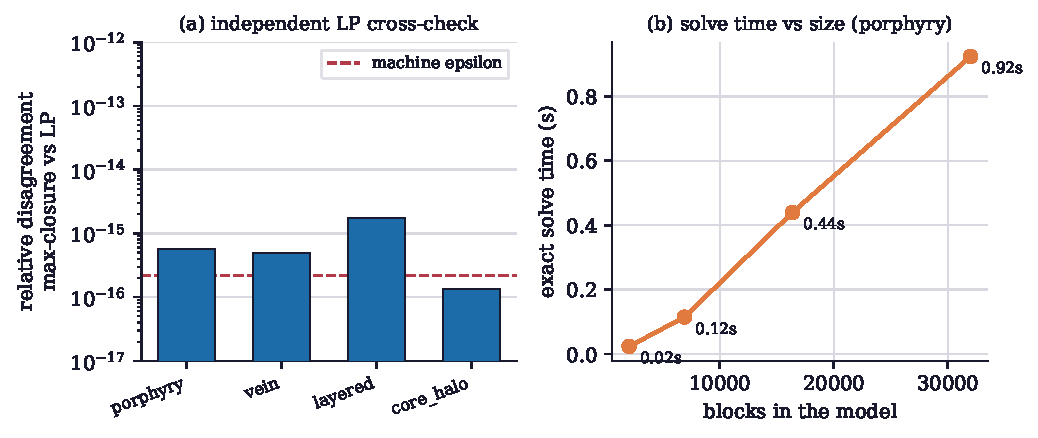
\includegraphics[width=0.99\columnwidth]{fig-scaling.pdf}
\caption{Solver validation, from the committed run. \textbf{(a)} Independent cross-check: on every archetype the
max-closure pit value agrees with the same instance solved as a linear program by SciPy HiGHS (an entirely
different algorithm) to relative $\sim\!10^{-15}$, machine precision (dashed line). \textbf{(b)} The exact solve
scales sub-second: $0.02$~s at $2{,}048$ blocks to $0.92$~s at $32{,}000$ blocks.}
\label{fig:scaling}
\end{figure}

\begin{figure}[!t]
\centering
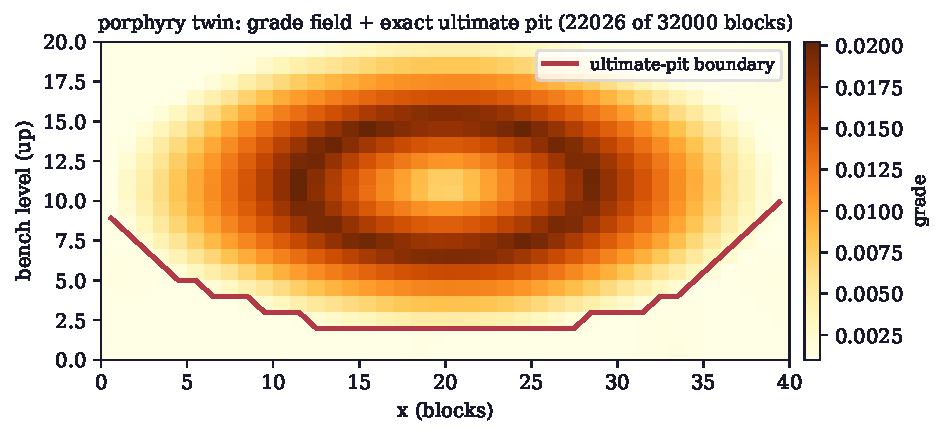
\includegraphics[width=0.99\columnwidth]{fig-pit.pdf}
\caption{A vertical cross-section of a porphyry twin: the grade field (the buried high-grade shell) with the
exact ultimate-pit boundary overlaid. The pit is a slope-feasible bowl whose walls step down bench by bench (the
discrete slope precedence), bottoming under the high-grade core, exactly the structure a real pit optimiser must
reproduce.}
\label{fig:pit}
\end{figure}

A synthetic benchmark is only as trustworthy as its stamped answer, so we do not merely assert the solver is
correct, we check it against an independent method. The ultimate-pit problem also has a linear-programming
formulation: maximise $\sum_b v_b x_b$ subject to $x_b \le x_p$ for every precedence relation and $0\le x_b\le
1$. Its constraint matrix is a network (incidence) matrix and hence totally unimodular, so the LP relaxation is
integral and its optimum equals the exact ultimate-pit value. We solve this LP with SciPy's HiGHS backend, a
completely different algorithm from the max-flow solver, on every archetype and compare
(Fig.~\ref{fig:scaling}a). The two agree to relative $10^{-15}$ (machine precision) on all four archetypes:
$5.7\times10^{-16}$ (porphyry), $4.9\times10^{-16}$ (vein), $1.7\times10^{-15}$ (layered), $1.4\times10^{-16}$
(core\_halo). This is an end-to-end check of the whole solve (the network construction, the flow, the residual
reachability, and the value identity), by a method that shares no code with it. It corroborates the package's
independent cross-check against a separate min-cut engine that reproduces the published MineLib optima
(newman1, zuck\_small, kd).

The exact solve is fast (Fig.~\ref{fig:scaling}b): from $0.02$~s at $2{,}048$ blocks to $0.92$~s at $32{,}000$
blocks, comfortably within the range a synthetic benchmark occupies. Table~\ref{tab:archetypes} lists the stamped
optima of the four archetypes at a common size, each with the solver's own value-identity gap (the residual of
the identity above), which sits at $10^{-7}$ or below, confirming the internal consistency of every stamped
answer. Figure~\ref{fig:pit} shows what an instance looks like: a porphyry cross-section with its exact pit, a
slope-feasible bowl that steps down bench by bench to the high-grade core.

\begin{table}[!t]
\centering
\caption{Stamped exact optima of the four archetypes ($24\!\times\!24\!\times\!12 = 6{,}912$ blocks, seed 11).
The value-identity gap is the solver's own self-check residual. \texttt{layered} is economic throughout at this
configuration, so its pit is the whole model.}
\label{tab:archetypes}
\footnotesize
\begin{tabular}{@{}l r r r r@{}}
\toprule
Archetype & Pit value & In pit & Fraction & Gap \\
\midrule
porphyry   & $4.71\times10^{8}$ & $4{,}631$ & $0.67$ & $6\times10^{-8}$ \\
vein       & $3.70\times10^{8}$ & $4{,}451$ & $0.64$ & $6\times10^{-8}$ \\
layered    & $1.46\times10^{9}$ & $6{,}912$ & $1.00$ & $2\times10^{-7}$ \\
core\_halo & $9.43\times10^{7}$ & $3{,}780$ & $0.55$ & $0$ \\
\bottomrule
\end{tabular}
\end{table}

\section{MineLib Format and the Stamped Twin}\label{sec:minelib}

An instance is emitted as a MineLib triplet plus a sidecar. The \texttt{.blocks} file lists per-block
coordinates and attributes, \texttt{.prec} the precedence in the compressed-sparse-row form MineLib uses, and
\texttt{.upit} the per-block economic value, so the triplet is byte-consumable by any MineLib reader. The
\texttt{.meta.json} sidecar carries the economics, the slope angle, and the \emph{stamped optimum} (pit value and
block count), so a solver under test reads the instance, computes its own pit, and compares against the stamped
answer with no licensed data anywhere in the loop. A whole instance with its certified optimum is one call:

\begin{lstlisting}[language=Python]
from oreblocks import make_twin
tw = make_twin("porphyry", dims=(20,20,10), seed=42)
tw.upit.pit_value, tw.upit.n_in_pit   # the exact optimum, stamped
tw.write("out/")   # -> .blocks / .prec / .upit / .meta.json
\end{lstlisting}

\section{Architecture and Availability}\label{sec:arch}

The package is small pure-Python modules (\texttt{grid}, \texttt{fields}, \texttt{economics},
\texttt{precedence}, \texttt{upit}, \texttt{minelib\_io}, \texttt{twins}) over NumPy storage, with no compiled
dependency, so it installs and runs anywhere Python does. It is deterministic given a seed, unit-tested (the
generators, the precedence, the solver's closure and identity checks, the MineLib round-trip), and MIT-licensed.
The downstream CAOS tools (a haulage simulator, a pit-forge twin generator, a dispatch bench) consume it for
geology-grounded, license-free instances. Source and the reproducible validation of this note are at
\url{https://github.com/fsantibanezleal/CAOS_OreBlocks}.

\section{Limitations}\label{sec:limits}

The scope is honest. \texttt{oreblocks} generates instances of the \emph{ultimate-pit} problem (the single-period
pit limit), not the constrained production-scheduling problem (CPIT/PCPSP) with capacities and time
periods~\cite{minelib}; those are a different, harder class. The deposits are geologically plausible synthetic
fields, not calibrated to any real ore body, and are labelled synthetic throughout. The economics is a standard
single-metal mine-vs-process model; multi-element or blending economics would need extension. The exact solver
targets the $10^3$--$10^5$-block range a benchmark generator occupies; for the multi-million-block industrial
models the specialised pseudoflow implementations~\cite{hochbaum} are the tool of choice, and \texttt{oreblocks}
writes MineLib format precisely so such solvers can consume its instances. None of these is hidden: the package
labels every instance synthetic and states what its stamped optimum does and does not certify.

\section{Conclusion}

\texttt{oreblocks} turns the shortage of redistributable ore-body benchmarks into a generator: seeded, synthetic,
geologically-structured block models of the MineLib nature, each stamped with its exact ultimate-pit optimum by
the classical max-closure/min-cut solve, emitted in MineLib format with the answer in a sidecar. The stamped
answer is trustworthy because it is checked, here, against an independent linear program to machine precision.
The value is a license-free, reproducible source of realistic pit-optimisation instances with certified optima,
for testing solvers, grounding simulators, and teaching, without touching licensed data.

\appendices
\section{Reproduction}\label{app:repro}

The validation is \texttt{manuscripts/ore-body-twins/figures/upit\_validation.py}: it builds each archetype,
solves the ultimate pit by the package's max-closure solver and independently as a HiGHS linear program, records
the agreement, the four stamped optima and the solve-time scaling, and extracts a porphyry cross-section. The
figure script reads those artifacts; the max-closure schematic is a hand-authored theme-aware drawing. Re-running
reproduces the cross-check ($10^{-15}$ agreement), Table~\ref{tab:archetypes}, and
Figs.~\ref{fig:scaling}--\ref{fig:pit}; the package is seeded and deterministic.

\balance

\begin{thebibliography}{00}

\bibitem{lg} H.~Lerchs and I.~F. Grossmann, ``Optimum design of open-pit mines,'' \emph{Transactions of the
Canadian Institute of Mining and Metallurgy}, vol.~68, pp.~17--24, 1965.

\bibitem{picard} J.-C. Picard, ``Maximal closure of a graph and applications to combinatorial problems,''
\emph{Management Science}, vol.~22, no.~11, pp.~1268--1272, 1976. doi:10.1287/mnsc.22.11.1268.

\bibitem{fordfulkerson} L.~R. Ford and D.~R. Fulkerson, ``Maximal flow through a network,'' \emph{Canadian
Journal of Mathematics}, vol.~8, pp.~399--404, 1956. doi:10.4153/CJM-1956-045-5.

\bibitem{dinitz} Y.~Dinitz, ``Dinitz' algorithm: The original version and Even's version,'' in \emph{Theoretical
Computer Science: Essays in Memory of Shimon Even}, LNCS 3895. Berlin: Springer, 2006, pp.~218--240.
doi:10.1007/11685654\_10.

\bibitem{hochbaumchen} D.~S. Hochbaum and A.~Chen, ``Performance analysis and best implementations of old and new
algorithms for the open-pit mining problem,'' \emph{Operations Research}, vol.~48, no.~6, pp.~894--914, 2000.
doi:10.1287/opre.48.6.894.12392.

\bibitem{hochbaum} D.~S. Hochbaum, ``The pseudoflow algorithm: A new algorithm for the maximum-flow problem,''
\emph{Operations Research}, vol.~56, no.~4, pp.~992--1009, 2008. doi:10.1287/opre.1080.0524.

\bibitem{minelib} D.~Espinoza, M.~Goycoolea, E.~Moreno, and A.~Newman, ``MineLib: A library of open pit mining
problems,'' \emph{Annals of Operations Research}, vol.~206, no.~1, pp.~93--114, 2013.
doi:10.1007/s10479-012-1258-3.

\bibitem{newman} A.~M. Newman, E.~Rubio, R.~Caro, A.~Weintraub, and K.~Eurek, ``A review of operations research
in mine planning,'' \emph{Interfaces}, vol.~40, no.~3, pp.~222--245, 2010. doi:10.1287/inte.1090.0492.

\end{thebibliography}

\end{document}
